\section{Conclusione}
In questa tesi sono stati presentati due modelli di controllo differenti, denominati PID e SMC. Attraverso l'utilizzo del software di modellazione Simulink, del tool "Embeded Coder Support Package for PX4 Autopilots" e il firmware PX4 con relativi strumenti per le simulazioni, è stato generato il codice sorgente e binario per l'hardware specifico scelto: CUAV\textregistered V5 Nano\textregistered. Attraverso la soluzione di alcune incompatibilità tra i vari strumenti, mediante l'utilizzo di script creati appositamente, è stato possibile effettuare diversi tipi di simulazioni di questi due modelli di controllo messi a confronto. \'E stato fatto inoltre un ulteriore confronto, attraverso l'utilizzo di modelli di simulazioni MIL precedentemente sviluppati, \cite{DesTestCarm}, degli stessi modelli utilizzando il profilo di missione più completo tra i precedentemente analizzati in SIL. \'E stato affrontato il problema di installazione del software nell'hardware selezionato, avvenuto con successo. Non è stato possibile effettuare le simulazioni PIL e i relativi confronti a causa dell'interfacciamento tra hardware e computer di sviluppo, riguardante i messaggi in uscita del controllore. 

\begin{figure}
	\centering
	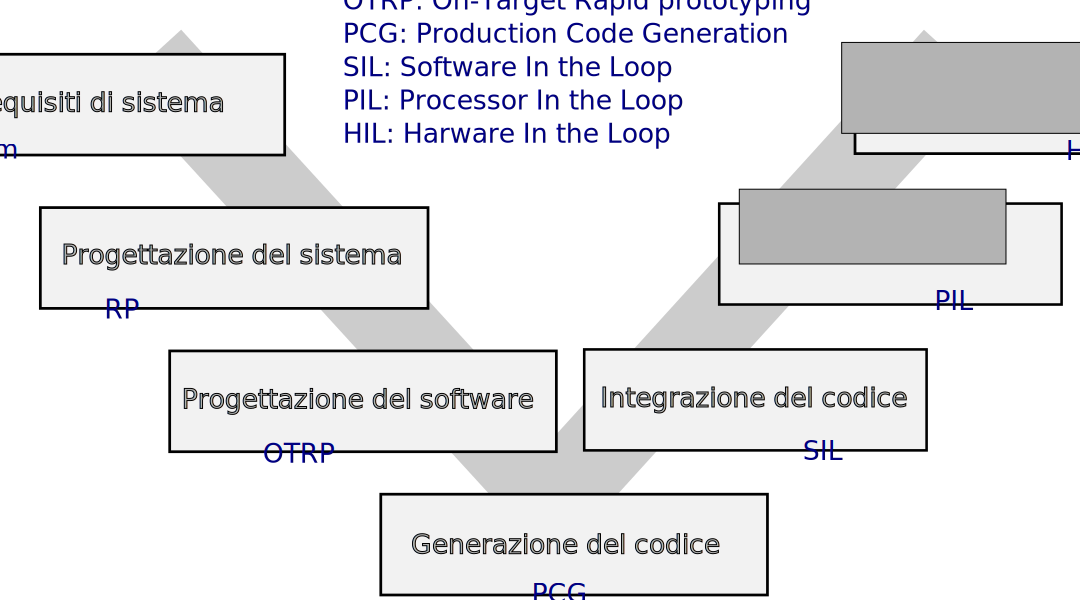
\includegraphics[width=0.9\textwidth]{Simulazioni/Figure/VSHAPE}
	\caption{Paradidma di progettazione model-based}
	\label{fig:VSHAPE}
\end{figure}

\'E stata dimostrata l'efficacia dell'approccio model-base, (\ref{fig:VSHAPE}), attraverso le varie simulazioni. I due modelli così progettati sono risultati effettivamente capaci di far volare autonomamente i quadrirotore nei diversi profili di missione trattati. Analizzando le simulazioni SIL effettuate, il controllore SMC risulta essere più prestante in termini di errore di posizione rispetto al modello di controllo PID, a discapito però di un maggior consumo di batteria, dovuto alla presenza di forti variazioni del comando fornito agli attuatori. Confrontando infine le simulazioni SIL con quelle effettuate in MIL, è stato validato attraverso l'analisi dei segnali e degli errori, l'effettiva coerenza dei risultati. Un analisi più approfondita ha mostrato come però sussistano differenze sostanziali in termini di campionamento del segnale è la necessita partendo dalle simulazioni MIL di effettuare anche una verifica attraverso SIL, per verificare la robustezza del sistema di controllo scelto. Il controllore SMC è risultato più robusto rispetto al controllore PID, che non ha una buona risposta in termine di comando del Position Control, proprio a causa del campionamento. Lo stesso effetto si verifica anche confrontando il risultati ottenuti nelle sue simulazioni, SIL e MIL, per quanto riguarda il controllo SMC, ma solo nel segnale PWM generato.

Negli sviluppi futuri di questo progetto, possono essere fatti diversi lavori aggiuntivi. La possibilità di effettuare simulazioni attraverso Gazebo permette di introdurre maggiore dettaglio nell'ambiente simulativo, di utilizzare sensori specifici e di implementare nuove funzionalità per il controllore. Lo stesso tipo di confronto effettuato in questa tesi può essere fatto per altri tipi di sistemi di controllo, verificandone l'effettiva robustezza. Per una più precisa analisi occorre inoltre collegare lo stesso ambiente Gazebo anche alla simulazione MIL, introducendo nel modello implementato in Simulink la porzione di algoritmo necessario a generale e gestire i messaggi utilizzati nativamente dal firmware PX4 utilizzando il protocollo MAVLink. Ulteriori indagini possono essere fatte modificando anche il generatore della traiettoria e del percorso, riducendo le repentine variazioni di velocità nella quale i sistemi presentati hanno maggiore difficoltà ad inseguire i segnali di riferimento. Per poter proseguire nel lavoro seguendo il paradigma di progettazione sopracitato, occorre indagare affondo su una soluzione per collegare efficacemente tutti gli strumenti fino ad ora disponibili, al fine di effettuare anche le simulazioni PIL necessarie. Concretamente occore poter superare la limitazione imposta dal tool "Embeded Coder Support Package for PX4 Autopilots", che non permette di utilizzare Gazebo come ambiente simulativo, ma solamente JMavSim, e nella nuova versione di MATLAB 2020b la modellazione del plant direttamente in Simulink. La soluzione utilizzando Gazebo come simulatore permetterebbe di poter accedere a funzionalità molto avanzate anche grazie all'utilizzo delle librerie di ROS. 